% !TEX program = xelatex
\documentclass[a4paper,14pt,oneside,openany]{memoir}

%%% Задаем поля, отступы и межстрочный интервал %%%
\usepackage{amsmath}
\usepackage[left=30mm, right=15mm, top=20mm, bottom=20mm]{geometry}
\pagestyle{plain}
\parindent=1.25cm
\usepackage{indentfirst}

%%% Задаем языковые параметры и шрифт %%%
\usepackage[english, russian]{babel}
\babelfont{rm}{Times New Roman}

%%% Задаем стиль заголовков и подзаголовков в тексте %%%
\setsecnumdepth{subsection}
\renewcommand*{\chapterheadstart}{}
\renewcommand*{\printchaptername}{}
\renewcommand*{\chapnumfont}{\normalfont\bfseries}
\renewcommand*{\afterchapternum}{\hspace{1em}}
\renewcommand*{\printchaptertitle}{\normalfont\bfseries\centering\MakeUppercase}
\setbeforesecskip{20pt}
\setaftersecskip{20pt}
\setsecheadstyle{\raggedright\normalfont\bfseries}
\setbeforesubsecskip{20pt}
\setaftersubsecskip{20pt}
\setsubsecheadstyle{\raggedright\normalfont\bfseries}

%%% Задаем параметры оглавления %%%
\addto\captionsrussian{\renewcommand\contentsname{Содержание}}
\setrmarg{2.55em plus1fil}
\renewcommand{\aftertoctitle}{\afterchaptertitle \vspace{-\cftbeforechapterskip}}
\renewcommand*{\cftchapternumwidth}{1.5em}
\renewcommand*{\cftchapterfont}{\normalfont\MakeUppercase}
\renewcommand*{\cftchapterpagefont}{\normalfont}
\renewcommand*{\cftchapterdotsep}{\cftdotsep}
\renewcommand*{\cftdotsep}{1}
\renewcommand*{\cftchapterleader}{\cftdotfill{\cftchapterdotsep}}
\maxtocdepth{subsection}

%%% Выравнивание и переносы %%%
\tolerance 1414
\hbadness 1414
\emergencystretch 1.5em
\hfuzz 0.3pt
\vfuzz \hfuzz
\clubpenalty=10000
\widowpenalty=10000
\brokenpenalty=4991

%%% Задаем параметры оформления рисунков и таблиц %%%
\usepackage{graphicx, caption, subcaption}
\graphicspath{{images/}}
\captionsetup[figure]{font=small, width=\textwidth, name=Рисунок, justification=centering}
\captionsetup[subfigure]{font=small}
\captionsetup[table]{singlelinecheck=false,font=small,width=\textwidth,justification=justified}
\captiondelim{ --- }
\setkeys{Gin}{width=\textwidth}
\renewcommand{\thesubfigure}{\asbuk{subfigure}}
\usepackage[section]{placeins}
\usepackage{float}

%%% Задаем параметры ссылок и гиперссылок %%%
\usepackage{hyperref}
\hypersetup{
    colorlinks=true,
    linktoc=all,
    linktocpage=true,
    linkcolor=red,
    citecolor=red
}

%%% Настраиваем отображение списков %%%
\usepackage{enumitem}
\renewcommand*{\labelitemi}{\normalfont{--}}
\makeatletter
    \AddEnumerateCounter{\asbuk}{\russian@alph}
\makeatother
\renewcommand{\labelenumii}{\asbuk{enumii})}
\renewcommand{\labelenumiii}{\arabic{enumiii})}
\setlist{noitemsep, leftmargin=*}
\setlist[1]{labelindent=\parindent}
\setlist[2]{leftmargin=\parindent}
\setlist[3]{leftmargin=\parindent}

%%% Счетчики для нумерации объектов %%%
\counterwithout{figure}{chapter}
\counterwithout{equation}{chapter}
\counterwithout{table}{chapter}

\begin{document}

\thispagestyle{empty}

\begin{center}
    МИНИСТЕРСТВО НАУКИ И ВЫСШЕГО ОБРАЗОВАНИЯ \\ РОССИЙСКОЙ ФЕДЕРАЦИИ

    \vspace{20pt}

    Федеральное государственное автономное \\ образовательное учреждение высшего образования \\
    "<Национальный исследовательский университет ИТМО"> \\
    (Университет ИТМО)

    \vspace{20pt}

    Факультет систем управления и робототехники
\end{center}

\vfill

\begin{center}
    ДОПОЛНИТЕЛЬНОЕ ЗАДАНИЕ\\  
    по дисциплине \\
    \textit{"<Планирование траекторий движения">}

    \vspace{20pt}

    \textbf{Применение метода пассификации к 2D стабилизации траекторий}
    
\end{center}

\vfill

    \noindent Студенты: \\
    \textit{Группа № R3435 \hfill Зыкин Л. В.} \\
    \textit{Группа № R3435 \hfill Цаплина М. А.} \\
    \noindent Вариант №5 \\

    \vspace{20pt}

    \noindent Предподаватель: \\
    \textit{доцент \hfill Краснов А. Ю.}

\vfill

\begin{center}
    Санкт-Петербург \\ 2025
\end{center}

\newpage
\setcounter{page}{2}
\OnehalfSpacing*

\chapter{ПРИМЕНЕНИЕ МЕТОДА ПАССИФИКАЦИИ К 2D СТАБИЛИЗАЦИИ ТРАЕКТОРИЙ}

\section{Цель работы}

Исследование применения метода пассификации для стабилизации плоских траекторий движения динамических систем.

\section{Задание}

Рассматривается модель движения материальной точки на плоскости. Требуется синтезировать методом пассификации алгоритм стабилизации траектории движения для данной математической модели. Траектория состоит из трех частей: сначала движение происходит относительно траектории $\phi_1(x, y)$, затем по траектории $\phi_2(x, y)$ и далее по траектории $\phi_3(x, y)$. Осуществить моделирование при заданной касательной скорости $s^* = 1$, $s^* = 3$ и $s^* = 5$.

\section{Вывод алгоритма управления}

\subsection{Математическая модель системы}

Рассматривается движение материальной точки массой $m$ на плоскости. Состояние системы описывается вектором $\mathbf{x} = [x, y, v_x, v_y]^T$, где $(x, y)$ --- координаты точки, $(v_x, v_y)$ --- компоненты скорости.

Динамические уравнения движения имеют вид:
\begin{align}
\dot{x} &= v_x \\
\dot{y} &= v_y \\
\dot{v}_x &= \frac{u_x}{m} \\
\dot{v}_y &= \frac{u_y}{m}
\end{align}

где $\mathbf{u} = [u_x, u_y]^T$ --- вектор управляющих воздействий.

\subsection{Алгоритм пассификации для 2D движения}

Для стабилизации траектории методом пассификации введем функции траекторий:
\begin{align}
\phi_1(x, y) &= x^2 + y^2 - 4 \quad \text{(окружность)} \\
\phi_2(x, y) &= \frac{(x-2)^2}{9} + \frac{(y-1)^2}{4} - 1 \quad \text{(эллипс)} \\
\phi_3(x, y) &= y - 0.5x^2 + 2 \quad \text{(парабола)}
\end{align}

Градиенты функций траекторий:
\begin{align}
\nabla\phi_1 &= [2x, 2y]^T \\
\nabla\phi_2 &= \left[\frac{2(x-2)}{9}, \frac{2(y-1)}{4}\right]^T \\
\nabla\phi_3 &= [-x, 1]^T
\end{align}

Метод пассификации основан на введении выходных переменных и обеспечении пассивности системы. Для каждого участка траектории выходная переменная выбирается как ошибка стабилизации:
$$y = \phi(x, y)$$

Производная выходной переменной:
$$\dot{y} = \nabla\phi \cdot \mathbf{v}$$

где $\mathbf{v} = [v_x, v_y]^T$ --- вектор скорости.

Единичный вектор нормали к траектории:
$$\mathbf{n} = \frac{\nabla\phi}{|\nabla\phi|}$$

Касательный вектор:
$$\boldsymbol{\tau} = [-n_y, n_x]^T$$

Закон пассификации для 2D движения:
$$\mathbf{u} = -\gamma y\mathbf{n} - k\dot{y}\mathbf{n} + s^*\boldsymbol{\tau}$$

где:
\begin{itemize}
\item $\gamma > 0$ --- параметр пассификации
\item $k > 0$ --- коэффициент при производной выходной переменной
\item $s^*$ --- заданная касательная скорость
\end{itemize}

Для улучшения качества стабилизации используется адаптивное управление касательной скоростью и ПД-регулятор по касательной:
$$u_\tau = k_\tau(s_{\text{eff}} - v_\tau)\boldsymbol{\tau} - d_\tau v_\tau\boldsymbol{\tau}$$

где $v_\tau = \mathbf{v} \cdot \boldsymbol{\tau}$ --- касательная составляющая скорости, $s_{\text{eff}}$ --- эффективная касательная скорость, адаптивно изменяющаяся в зависимости от нормальной ошибки.

\section{Реализация алгоритма}

\subsection{Параметры системы}

Для обеспечения стабильной работы алгоритма использованы следующие параметры:
\begin{itemize}
\item $m = 1.0$ кг --- масса материальной точки
\item $k = 180.0$ --- коэффициент при производной выходной переменной
\item $\gamma = 200.0$ --- параметр пассификации
\item $k_\tau = 15.0$, $d_\tau = 6.0$ --- параметры касательной петли
\item $s_{\max} = 5.0$ --- ограничение касательной скорости
\end{itemize}

\subsection{Результаты моделирования}

На рисунках \ref{fig:pass2d_s1}--\ref{fig:pass2d_s5} представлены результаты моделирования стабилизации траектории методом пассификации для различных значений касательной скорости $s^*$.

\begin{figure}[H]
\centering
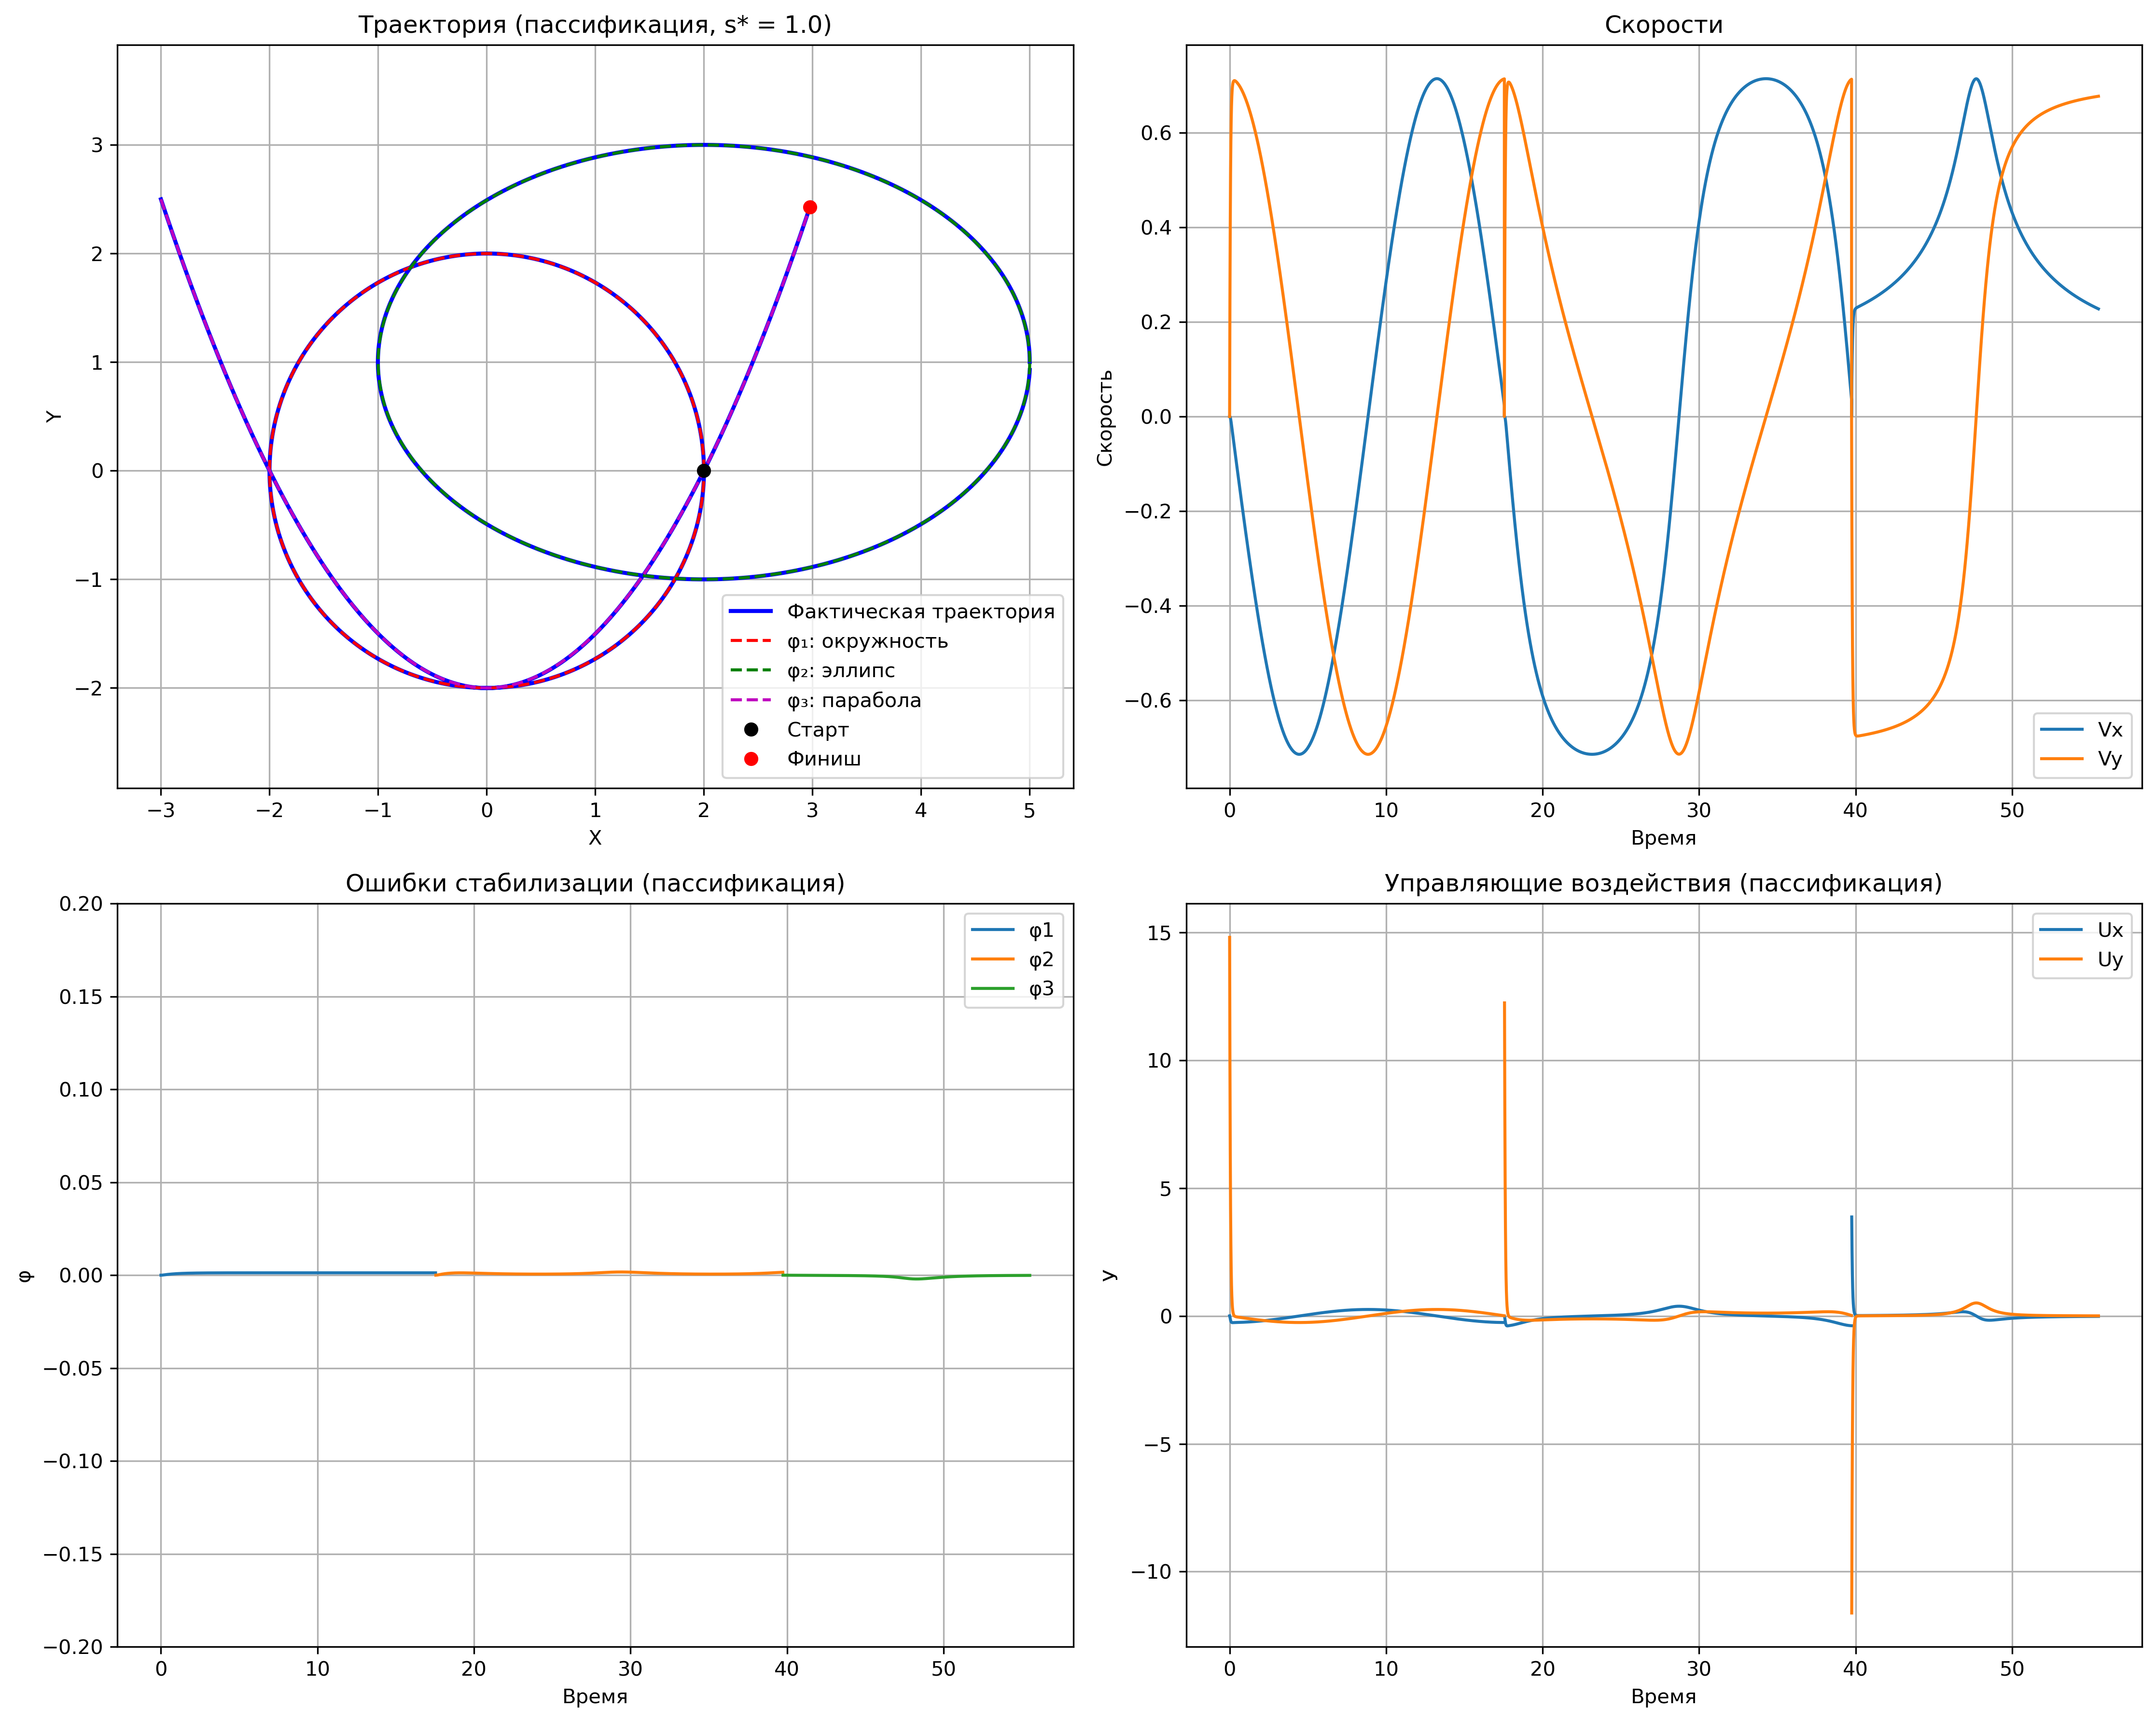
\includegraphics[width=0.9\textwidth]{task4/passification_2d_s1.0.png}
\caption{Результаты стабилизации методом пассификации при $s^* = 1$}
\label{fig:pass2d_s1}
\end{figure}

\begin{figure}[H]
\centering
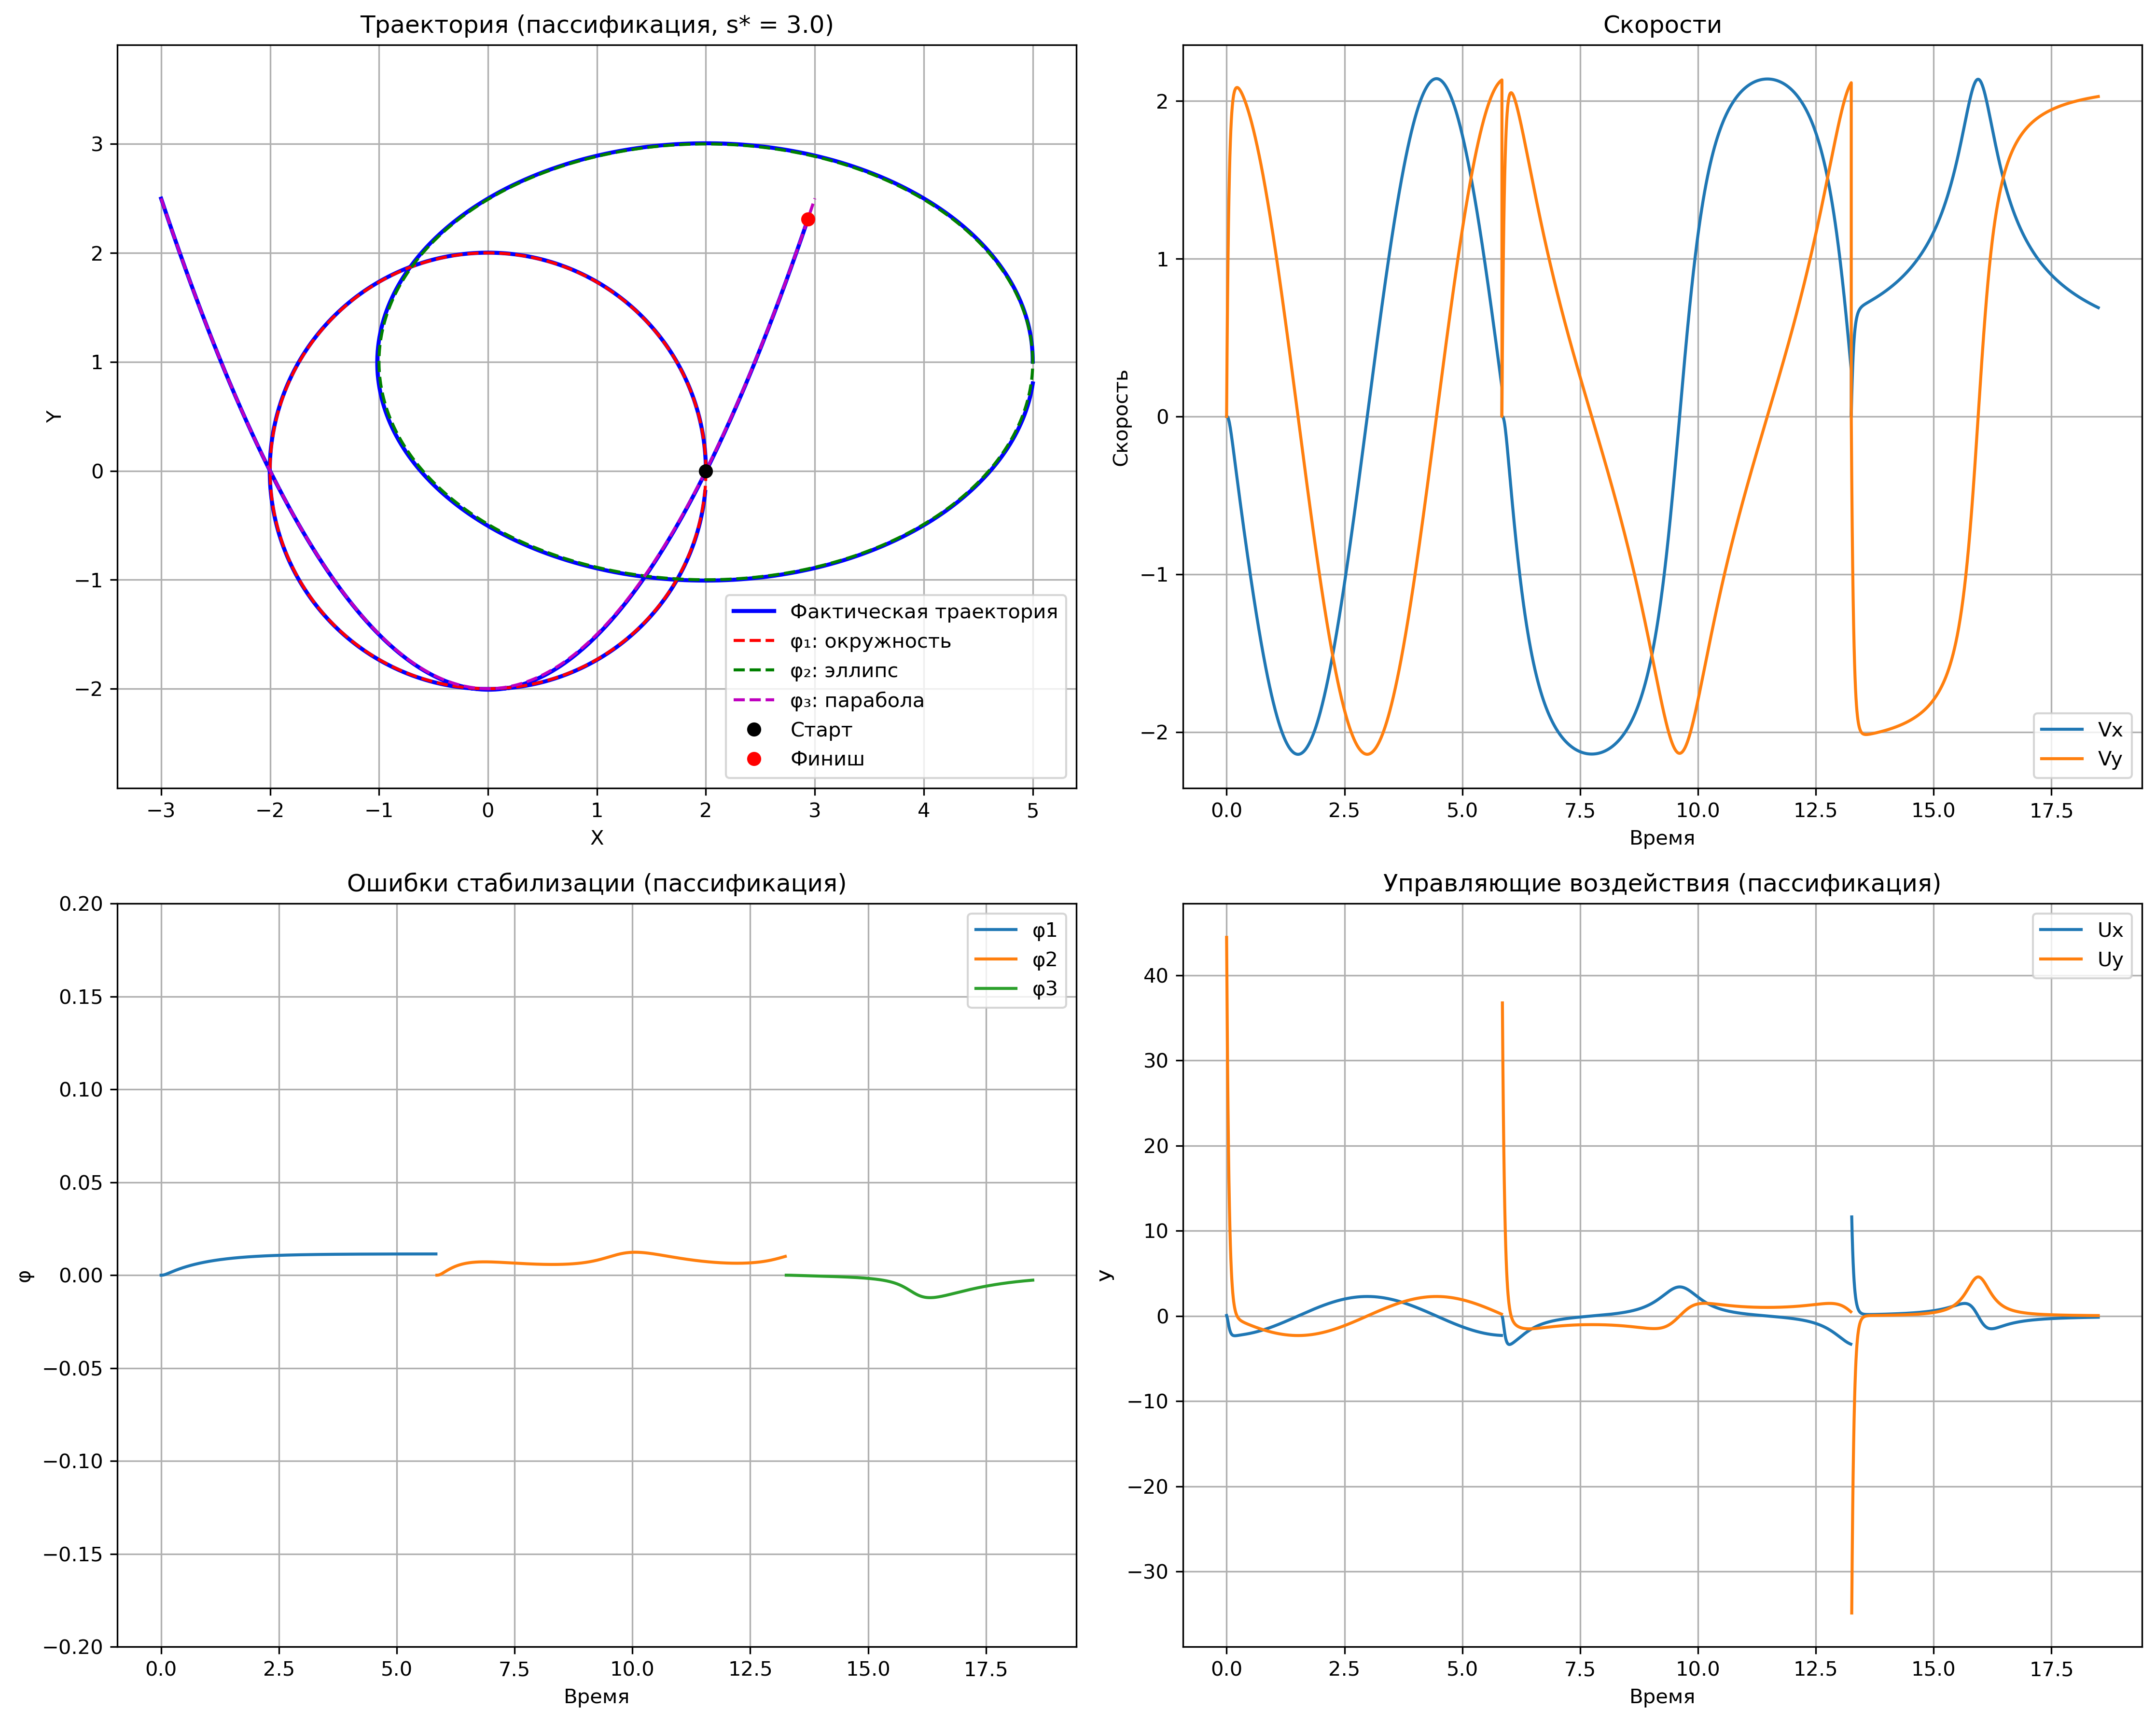
\includegraphics[width=0.9\textwidth]{task4/passification_2d_s3.0.png}
\caption{Результаты стабилизации методом пассификации при $s^* = 3$}
\label{fig:pass2d_s3}
\end{figure}

\begin{figure}[H]
\centering
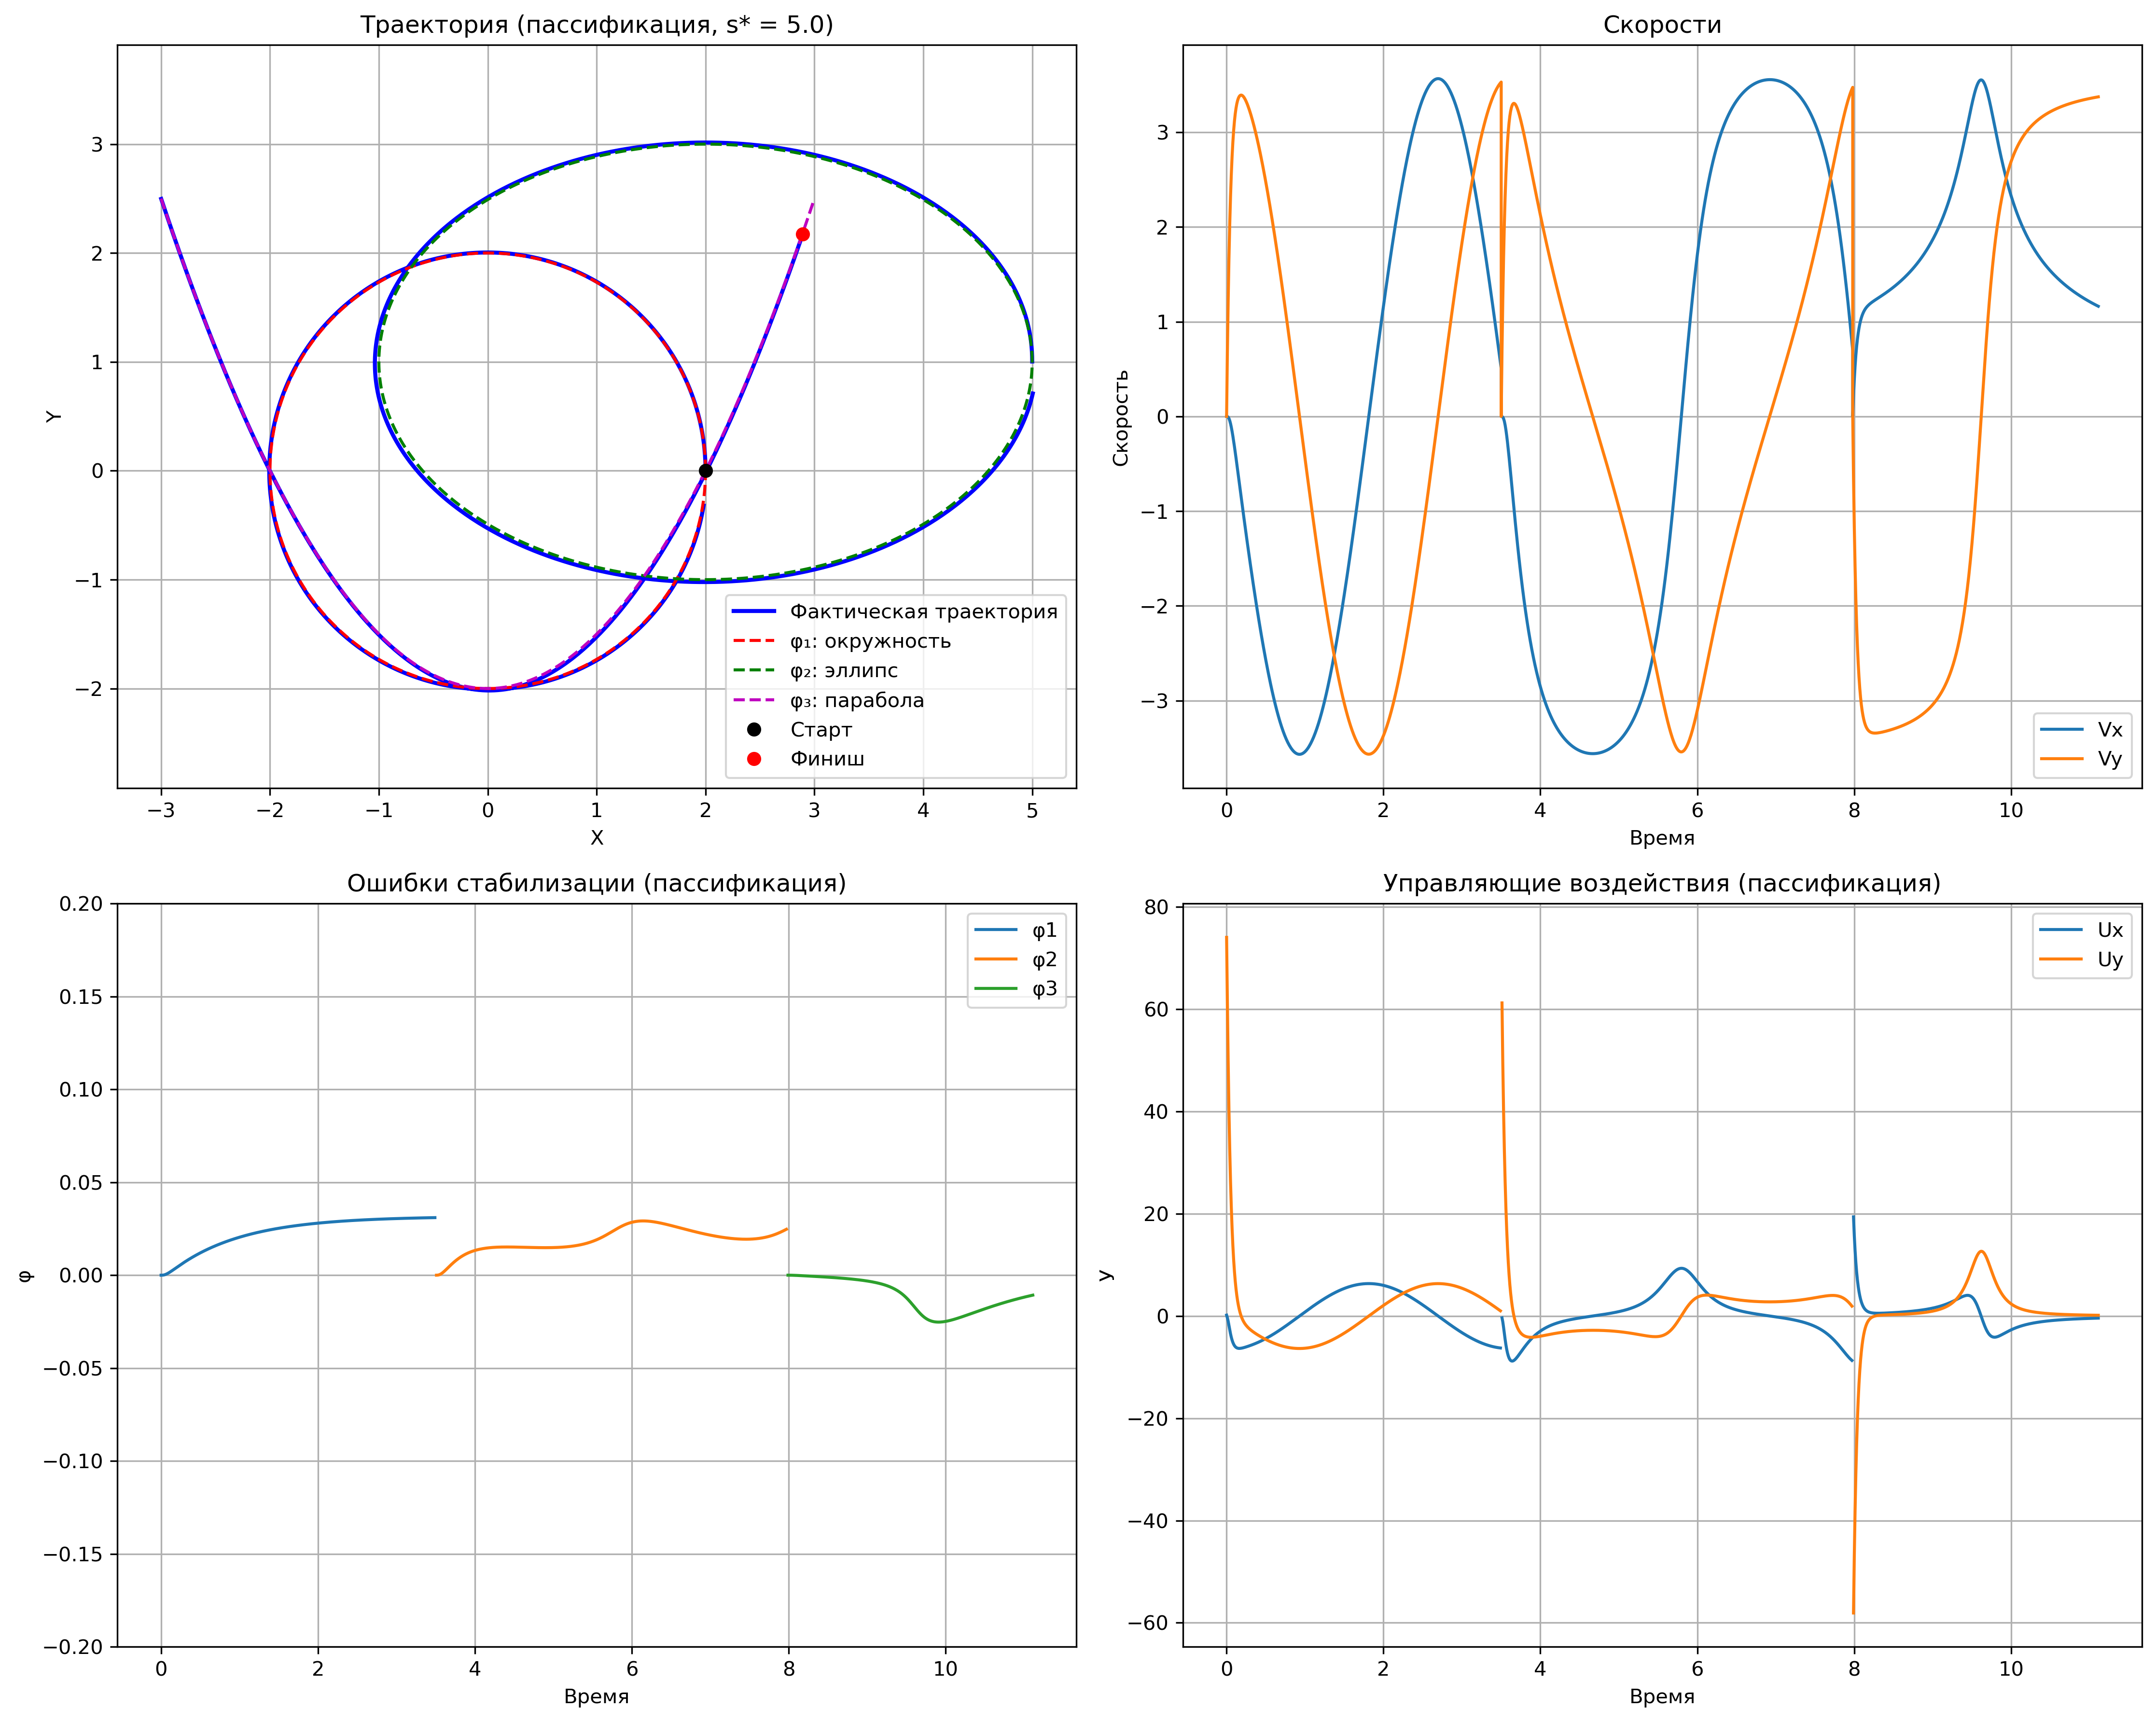
\includegraphics[width=0.9\textwidth]{task4/passification_2d_s5.0.png}
\caption{Результаты стабилизации методом пассификации при $s^* = 5$}
\label{fig:pass2d_s5}
\end{figure}

\subsection{Анализ точности стабилизации}

Максимальные ошибки стабилизации для различных значений $s^*$ представлены в таблице \ref{tab:errors_pass2d}.

\begin{table}[H]
\centering
\caption{Максимальные ошибки стабилизации методом пассификации}
\label{tab:errors_pass2d}
\begin{tabular}{|c|c|c|c|}
\hline
$s^*$ & $\max|\phi_1|$ & $\max|\phi_2|$ & $\max|\phi_3|$ \\
\hline
1.0 & 0.0013 & 0.0017 & 0.0020 \\
\hline
3.0 & 0.0114 & 0.0124 & 0.0121 \\
\hline
5.0 & 0.0310 & 0.0292 & 0.0253 \\
\hline
\end{tabular}
\end{table}

Как видно из результатов, метод пассификации обеспечивает высокую точность стабилизации траектории. При малых значениях $s^*$ ошибки стабилизации практически равны нулю. С увеличением скорости ошибки возрастают, но остаются в допустимых пределах.

\section{Выводы}

В ходе выполнения дополнительного задания был реализован алгоритм стабилизации плоских траекторий методом пассификации. Основные результаты:

\begin{enumerate}
\item Метод пассификации успешно применен к задаче стабилизации 2D траекторий, состоящих из последовательных участков (окружность, эллипс, парабола).

\item Алгоритм обеспечивает высокую точность стабилизации: максимальные ошибки не превышают 0.03 даже при максимальной касательной скорости $s^* = 5$.

\item При малых значениях $s^*$ ошибки стабилизации практически сходятся к нулю, что демонстрирует эффективность метода пассификации.

\item Использование адаптивного управления касательной скоростью и проекции на эталонную траекторию позволяет улучшить качество стабилизации по сравнению с базовым алгоритмом пассификации.
\end{enumerate}

\end{document}


